\section{Selection error grows with the search space}
\label{sec:C09:selection}
More candidates increase coverage but also expose the selector to more opportunities for error. Let candidate $i$ have true utility $u_i$ and estimated score $\widehat u_i=u_i+e_i$. Suppose each error has a sub-Gaussian tail $P(|e_i|>t)\leq2\exp[-t^2/(2\sigma^2)]$. A union bound gives simultaneous error at most $t=\sigma\sqrt{2\log(2K/\delta)}$ with probability at least $1-\delta$ across $K$ candidates. Independence is not needed for this union bound, though the marginal tail assumption must hold for the evaluated candidates.

If $\widehat i$ maximizes estimated score and $i^*$ maximizes true utility, simultaneous error control yields $u_{i^*}-u_{\widehat i}\leq2t$. Add and subtract the two estimated scores; their difference is nonpositive by selection, leaving two bounded errors. This elementary deduction formalizes a selection effect: the score accuracy required for a fixed regret tolerance becomes stricter as the candidate set grows. A method can discover better candidates while selecting a worse final answer. The correct diagnosis separates coverage, recognition, and final selection rather than treating all failure as insufficient generation quality. For a selector restricted to the generated candidate set, let $C$ be the event that the set contains a correct artifact and $A$ the event that the selected artifact is correct. Then $A\subseteq C$ and
\begin{equation}
 \Pr(A)=\Pr(C)\Pr(A\mid C)\leq\Pr(C),
 \qquad\Pr(C)>0.
\end{equation}
This separates generator coverage from conditional selection success. A selector allowed to create a new answer changes the candidate set and must be evaluated under that expanded boundary; the inequality cannot be transferred silently to a different pipeline.

The assumptions deserve scrutiny in adaptive search. Candidates are proposed in response to earlier scores, so an error bound established on random unselected examples may not transfer. A reward model can be exploited by repeatedly searching for high-scoring artifacts. Calibration on ordinary completions is therefore insufficient evidence of robustness under optimization. Evaluate the judge on planner-selected candidates, preserve hidden tests, and record whether a correct candidate appeared but was rejected. These records explain whether additional compute should be spent on generation, verification, or a different scoring objective.

Binary validators have a related multiple-testing problem. If each invalid candidate has conditional false-acceptance probability at most $\epsilon$ given the prior search history, the probability of at least one false acceptance among at most $K$ checks is at most $K\epsilon$. This conservative bound does not require independent checks. It does require the conditional error guarantee, which adversarially selected candidates can violate. A validator with a small average false-positive rate can become unreliable when an optimizer targets its blind spots. Increasing the sample budget without strengthening verification can therefore worsen accepted-output quality.

\subsection{A calculated selector with an imperfect validator}
Assume independent candidates are correct with probability $p$, and a validator accepts correct candidates with probability $s$ and incorrect candidates with probability $f$. Its acceptance probability is $q=ps+(1-p)f$. Conditional on acceptance, correctness is $ps/q$ when $q>0$. If the system returns the first accepted candidate, unbounded retries have the same accepted-output correctness and mean attempt count $1/q$. More attempts increase the chance of returning something; they do not improve the precision of this stationary acceptance rule. This deduction separates availability from correctness and prevents a retry loop from being described as verification improvement.

For hypothetical $p=0.3$, $s=0.9$, and $f=0.1$, acceptance is $0.34$, accepted-output correctness is approximately $0.7941$, and the mean number of unbounded attempts is approximately $2.9412$. With four attempts, the chance of any acceptance is $1-0.66^4\approx0.8103$. These are calculated examples, not measured characteristics of a model judge. They assume the validator's errors and the candidate distribution remain stationary, with fresh independent trials. Real adaptive search often violates precisely these assumptions because later candidates are chosen to exploit previous scores.

{\small\setlength{\tabcolsep}{3pt}
\begin{table}[!htbp]
\centering
\caption{Calculated behavior of the hypothetical imperfect selector.}\label{tab:C09:selector}
\begin{tabular}{L{37mm}L{30mm}L{39mm}}

\toprule Quantity & Value & Boundary\\\midrule
Per-attempt acceptance & 0.34 & Includes false acceptance.\\
Correctness given acceptance & 0.7941 & Does not improve with stationary retries.\\
Mean unbounded attempts & 2.9412 & No deadline or changing environment.\\
Acceptance within four attempts & 0.8103 & Availability, not verified success.\\
\bottomrule
\end{tabular}
\end{table}
}

The example also identifies which intervention matters. Reducing the false-positive rate can improve accepted-output correctness substantially even if candidate generation does not improve. Increasing sensitivity can reduce wasted rejection of good candidates. Improving $p$ helps both coverage and precision, but may cost a larger model or more computation per attempt. A scientific comparison should measure all three rather than crediting the generator for a better validator or describing a more permissive validator as improved reasoning. When true labels are expensive, audit a stratified sample of accepted and rejected candidates, with sampling weights that permit reconstruction of the desired rates.

Optional stopping requires care in evaluation. If the system repeatedly checks until a favorable score appears, reporting the final score without the number of checks introduces selection bias. The final artifact should be judged by a held-out acceptance procedure that was not used to guide the search. This does not require that every verifier be secret forever; it requires separation between optimization feedback and the evidence used to estimate generalization. For executable tasks, hidden tests and independent specification review can serve complementary roles. Neither resolves an ambiguous task specification automatically.

Stateful tasks make the stationary example especially fragile. A rejected candidate may have already changed files or consumed a one-time token. A repeated browser action can alter the environment even when the judge says it failed. The selector should either operate on isolated candidate artifacts before execution or explicitly model these transitions. Retaining the complete operation history makes it possible to distinguish improved solution search from repeated interaction with a gradually changing task. This distinction is essential when comparing self-correction, sampling, and planning under the same nominal attempt budget.



Figure~\ref{fig:C09:coverage-selection} isolates the mechanism and its stated information boundaries.
\begin{figure}[!htbp]
\centering
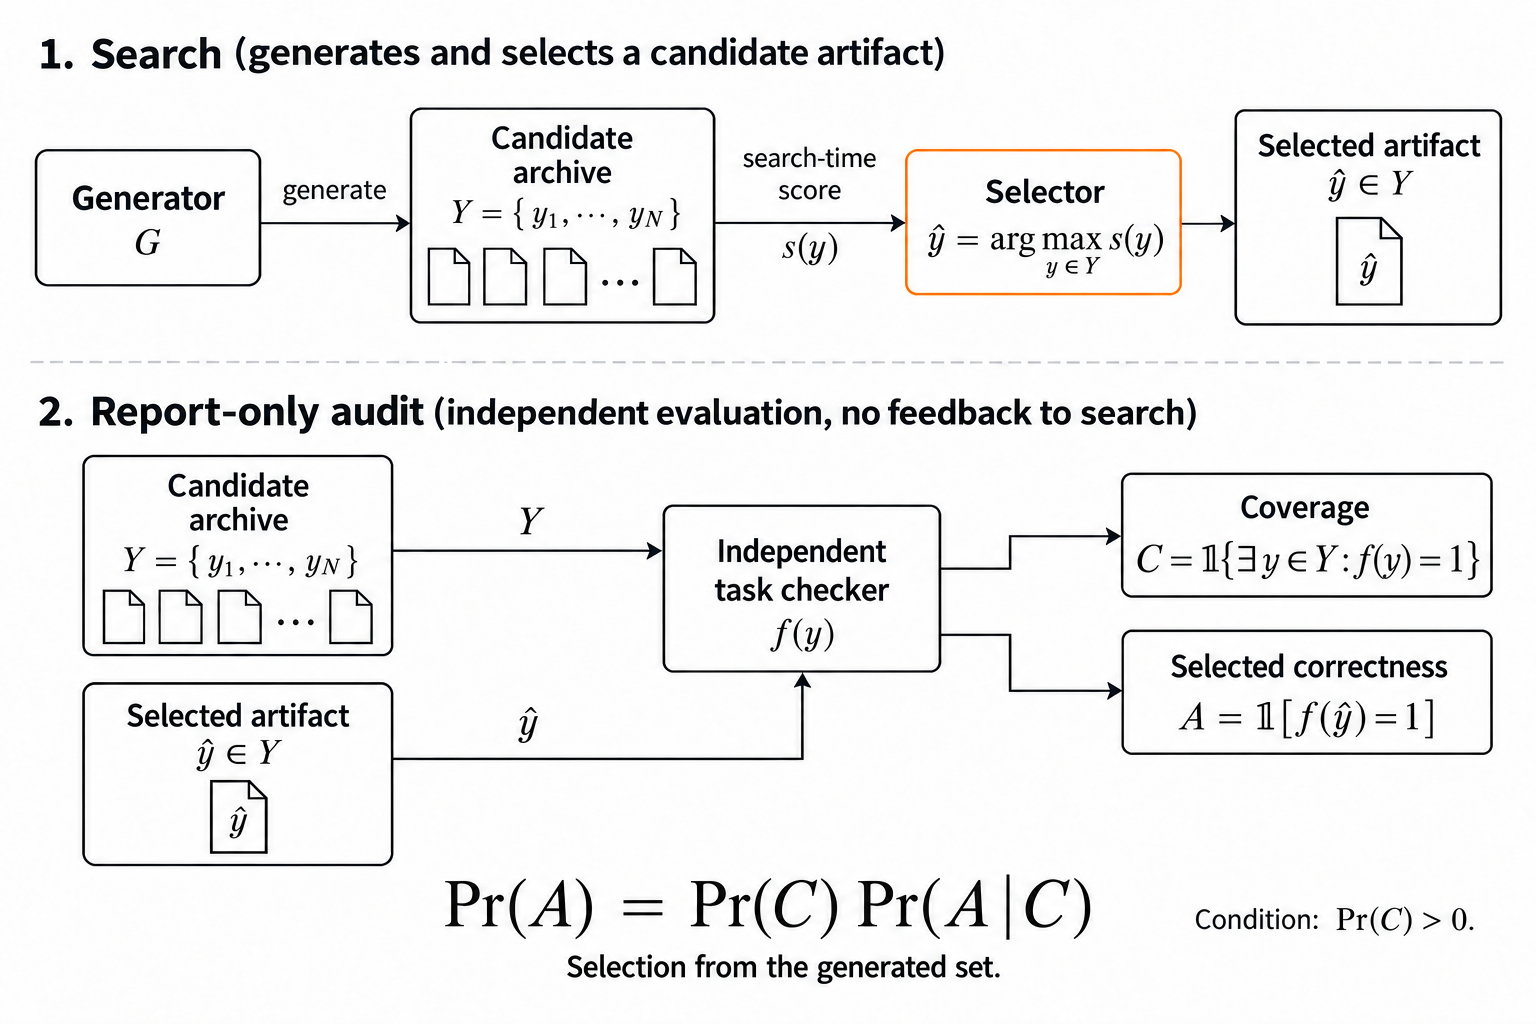
\includegraphics[width=\linewidth]{book/figures/assets/F09review.png}
\caption{Search-time scores and report-only acceptance labels serve different roles. Under one fixed acceptance map $f$, the displayed indicators satisfy $A\le C$ when $\widehat y\in\mathcal{Y}$. The probability notation abbreviates $\Pr(A=1)$ and $\Pr(C=1)$; the decomposition requires $\Pr(C=1)>0$. A fallible checker measures its declared acceptance criterion. Pruning attribution additionally requires stage-labelled candidate records; the selected artifact alone is insufficient.}
\label{fig:C09:coverage-selection}
\end{figure}
